\texit{Определение} Адаптер называется низкоранговое дополнение
к основной нейросети, выполняющее адаптацию на конкретную задачу.

Для любых матрица $A$ и $B$ выполняется
\begin{equation}
    \rang(𝐴𝐵) \le \min\left(\rang(𝐴),\rang(𝐵))
\end{equation}
   
Низкоранговый адаптер Lora работает путем сжатия 
параметров модели с использованием низкоранговых матриц. 
Основная идея заключается в том, 
чтобы аппроксимировать исходные параметры модели с
помощью матриц меньшего ранга, что позволяет снизить объем памяти.
Это позволяет снизить объем памяти,необходимый для хранения параметров и ускорить вычисления. 
\begin{figure}[h]
    \centering
    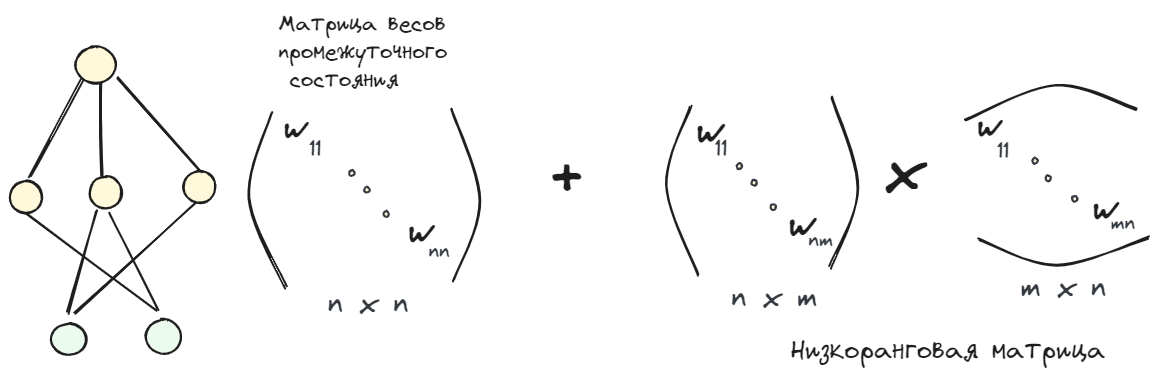
\includegraphics[width=0.5\textwidth]{assets/ml/adapter/adapter.excalidraw.png}
    \caption{Модель адаптера \text{Lora} \cite{hu2021lora}}
    \label{sd_learning}
\end{figure}

Наиболее популярным вариантом адаптера является Lora \cite{hu2021lora}:
\begin{equation}
    \hat{W} = W + AB,
\end{equation}
где  $AB$ - низкоранговая матрица, полученная произвелением 
матриц $A$ размерности \( m \times r \) и  $B$ размерности \( r \times n \)?
где \( r \) - это ранг аппроксимации.